\section{Datapath}
This section describes the data-path and its internal elements. The data-path is the component that connects the pipeline components within itself as well as with CPU inputs and outputs and the control-path.

This MIPS implementation works with a 5 stage pipeline in order to achieve a fast clock. The data-path consists of instruction fetch, instruction decode, execution, memory stage and write-back.
The data-path controls the information flow from one pipeline stage to the next with registers. 
These writing process occur on the positive edge of the clock when the pipeline stage input from the control-path, so that the registers forwards information synchronously. 
The data-path forwards the control-path signals asynchronously, contrary to the pipeline to pipeline signals.



\begin{figure}[h!]
  \centering
  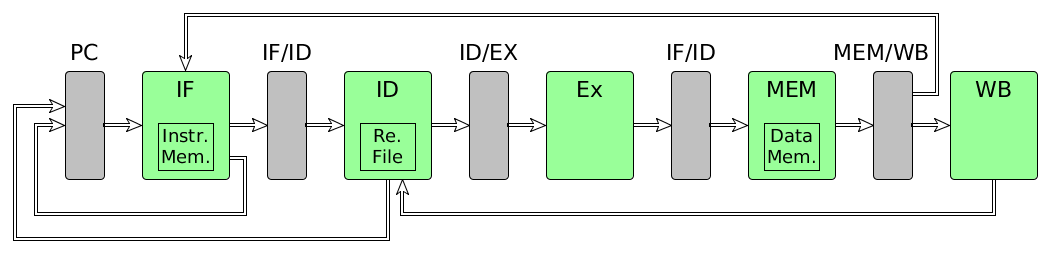
\includegraphics[width=0.8\textwidth]{figure/datapath.png}
  \caption{Data-path pipeline}
  \label{fig:datapath}
\end{figure}

The program counter (PC) is programmed into the data-path. Its function is the store the current program address, which is mostly counted up.
It has a multiplexer controlled by the control-path to choose the input. The two possible inputs are to count up (PC+4) from instruction fetch
and the jump or branch from instruction decode. The control-path chooses always the instruction decode input in the case of jump or branch. 


The following subsections describe the pipeline components as well as its functions and IOs. 

\subsection{Instruction fetch}
This first block of the pipeline is the instruction fetch. The main task of this block is to fetch the next instruction and relay it to the pipeline. 

The program counter is a 32-bit input, which is directly outputted as instruction address to fetch an instruction. The instruction fetch inputs the program memory's instruction data, 
with the 32-bit instruction. This value is directly forwarded to the pipeline. The memory word is one byte long, but each instruction read operation retrieves four bytes or the 32-bit
word.

The program counter is also incremented by four, because the used memory is 8-bit long, pointing to the next valid instruction. This incremented value is given back to PC.
\subsection{Instruction decode}
The second block of the pipeline if the instruction decode. Its main tasks are to divide the instruction into its pieces, manage the register file and manage branches.

The main input is the instruction from the instruction fetch stage. This instruction is 32-bit long and can be of three types. These are shown in \autoref{tab:instr type} \cite{mips32}.

\begin{table}[h!]
	\centering
	 \caption{MIPS instruction types}	
	\begin{tabular}{ccccccc}
		\toprule[2pt]
		\textbf{Type} & \multicolumn{6}{c}{\textbf{format (bits) }}   \\
		\toprule[2pt]
		R & opcode (6) & rs (5) & rt (5)   & rd (5) & shat (5) & funct (6) \\
		I & opcode (6) & rs (5) & rt (5)   & \multicolumn{3}{c}{ immediate (16)} \\
		J & opcode (6) & \multicolumn{5}{c}{ address (26)} \\	
		\bottomrule[2pt]
	\end{tabular} 
	\label{tab:instr type}
\end{table}

The \textbf{opcode} indicates the operation or arithmetic family of operations. Opcode equals zero are the R-type operations. The field \textbf{funct} provides an specific operation.
\textbf{rs}, \textbf{rt} and \textbf{rd} provide sources or destinations register addresses. \textbf{shamt} indicates the shift amount for shift operations. \textbf{immediate} carries
a relative address or constant, which is zero or sign extended to 32-bits. \textbf{address} is an absolute address.

The main outputs are register A, register B, shift, regdest, immediate and IP. Other than IP, all outputs depend on the instruction decoding. 
Register A contains always the value that is contained in the register given by the source register field (instruction's sub-vector 25-21). 
Register B likewise always contains the value of the register given by the R-type-instruction's field for the target register (instruction's sub-vector 20-16). 
Immediate always contains the lower half of the instruction with a signed extension. 

Regdest has to be chosen by the control path. It can be either the target 
register field or the R-type's destination register field or 31, which was originally implemented for jump-and-link- or branch-and-link-instructions, but rendered pointless
by the more complex branch logic and write-back functionality for register 31. Shift also must be chosen by the control path. It can be set to the R-type-instruction's shift-field, 
to 16 or to 0. 

The execution stage chooses the signals necessary for an operation using two multiplexers so if any output yields a nonsensical value is is simply not used.

\subsubsection{Register File}
The register file is a set of 32 general purpose 32-bit registers. These have the advantage, comparing to the ram memory, that they can always be accessed within one clock cycle.
The access to these registers is made with five bits, which allows multiple registers to be referenced per instruction. All loaded memory values are stored in a register
for later use.

The registers are numbered from \$0 through \$31. There is also a convention for using these registers, which must be enforced by assembly language and follow \autoref{tab:mips registers} 
\cite{regfiles}:

\begin{table}[h!]
	\centering
	 \caption{MIPS registers}	
	\begin{tabular}{ccl}
		\toprule[2pt]
		\textbf{Register Number} & \textbf{Conventional Name} &\textbf{Usage}  \\
		\toprule[2pt]
		\$0 & \$zero & Hard-wired to 0 \\
		\$1 & \$at & Reserved for pseudo-instructions \\
		\$2 -\$3 & \$v0, \$v1 & Return values from functions \\
		\$4 - \$7 & \$a0 - \$a3 & Arguments for functions - not preserved by subprograms \\
		\$8 - \$15 & \$t0 - \$t7 & Temporary data, not preserved by subprograms \\
		\$16 - \$23 & \$s0 - \$s7 & Saved registers, preserved by subprograms \\
		\$24 - \$25 & \$t8 - \$t9 & More temporary registers, nor preserved by subprograms  \\
		\$26 - \$27 & \$k0 - \$k1  & Reserved for kernel. Dot not use. \\
		\$28 & \$gp & Global Area Pointer (base of global data segment) \\
		\$29 & \$gp & Stack pointer \\
		\$30 & \$sp & Frame Pointer \\
		\$31 & \$ra & Return Address \\
		\bottomrule[2pt]
	\end{tabular} 
	\label{tab:mips registers}
\end{table}

This implementation of MIPS does not have a FPU. In case of FPUs another 32 32-bit register set is used.

The register file is written on the clock's negative edge with write-back information. The register file require a 5-bit destination register address and the 32-bit word to be written into the register. 
Additionally there is the possibility to write to register 31. On every rising clock cycle, an internal write-back flag is checked. If it was set by another process, 
the value of the internal write-back register is copied to register 31. This bypasses some pipeline stages, but makes control path design a little easier.
\subsubsection{Branch Logic}
The branch and jump instructions require just one clock between instruction fetch and the jump itself. Due to this constrain, there is the need of a branch logic inside
the instruction decode part. The output of this operation is the next instruction address for PC. 

On the jump command, PC will receive the jump value. 
In case of a branch, PC will receive either the branch value or PC+4, depending on the instruction decode decision. This behavior allows for the control-path always to 
activate the instruction decode input in cases of jumps and branches. If a Jump-and-link- or a branch-and-link-instruction is detected, the branch logic writes the last 
program counter to the internal write-back register and sets the internal write-back flag to 1 to signal a necessary copy operation to the register bank. 
It evaluates the flag and treats the internal write-back register as described above.
\subsubsection{Forwarding}
Often calculated or memory read values are used in the following instructions. Due to the pipeline, the values are not ready in the register file, causing a data hazard. In order to avoid this conflict
a data forwarding system is integrated. The data forwarding provide separated inputs for the 5-bit destination register address and the 32-bit word for the ALU, memory stage and write-back. 
If the destination register address in one of this stages is equal to an address used in the current instruction decode phase, the value of the register bank is replaced by a forwarded value. 
The forwarding system takes care to always use the most recent value. For example, if both write-back and execution stage contain the same destination address, 
the execution stage's value is forwarded because the value that has to be written to that destination register was changed by the instruction in the execution stage after 
it was changed by the instruction in the write-back stage, so the value contained in the execution stage is the most recent.


\subsection{Execution}
This stage of the pipeline takes care of the actual mathematical operations. It provides two main multiplexers, one for each value input of the ALU.
The inputs of the first multiplexer are the zero padded shift input, the number four (32-bit) and the register A from instruction decode. The second multiplexer provides register B, 
the immediate value and IP as inputs.

Both multiplexers are controlled by the control-path.
\subsection{Memory Stage}
The memory stage is the fourth block of the pipeline and has the main task of fetch or save in the memory. 

For memory operations the execution stage outputs two 32-bit values: aluResult\_in, which works as the memory address, and data\_in, which is data to be written in the memory. 
On read operations, the data\_to\_cpu input delivers the 32-bit memory value.

This stage has one multiplexer choosing the pipeline stage output from aluResult\_in or data\_to\_cpu.
\subsection{Write-back}
This write-back stage is the fifth and last stage of the pipeline. Its main task is just to hold the calculated values, as well as the values read from the memory 
so they can be written the register file.
